\colorlet{ind}{black}
\colorlet{dep}{gray!50!white}
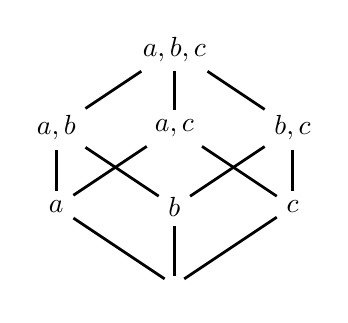
\begin{tikzpicture}
  \draw (0, 0)    node (o) {$\varnothing$};
  \draw (-1.5, 1) node (a) {$\setprn{a}$};
  \draw (0, 1)    node (b) {$\setprn{b}$};
  \draw (1.5, 1)  node (c) {$\setprn{c}$};
  \draw (-1.5, 2) node (ab) {$\setprn{a, b}$};
  \draw (0, 2)    node (ac) {$\setprn{a, c}$};
  \draw (1.5, 2)  node (bc) {$\setprn{b, c}$};
  \draw (0, 3)    node (abc) {$\setprn{a, b, c}$};
  \draw[line width=1pt] (abc) -- (ab);
  \draw[line width=1pt] (abc) -- (ac);
  \draw[line width=1pt] (abc) -- (bc);
  \draw[line width=1pt] (ac) -- (a);
  \draw[line width=1pt] (ac) -- (c);
  \draw[line width=1pt] (ab) -- (a);
  \draw[line width=1pt] (ab) -- (b);
  \draw[line width=1pt] (bc) -- (b);
  \draw[line width=1pt] (bc) -- (c);
  \draw[line width=1pt] (a) -- (o);
  \draw[line width=1pt] (b) -- (o);
  \draw[line width=1pt] (c) -- (o);
\end{tikzpicture}
